%
% main.tex -- Paper zum Thema <helmholtz>
%
% (c) 2020 Autor, OST Ostschweizer Fachhochschule
%
% !TEX root = ../../buch.tex
% !TEX encoding = UTF-8
%
\chapter{Helmholtz-Zerlegung\label{chapter:helmholtz}}
\kopflinks{Helmholtz-Zerlegung}
\begin{refsection}
\chapterauthor{Joël Rechsteiner}

Im Mittelpunkt in diesem Kapitel steht die Helmholtz-Zerlegung.
Anhand eines Beispiels aus der Physik in der Akustik aus dem Paper
\cite{helmholtz:paper}
wird eine Anwendung der Helmholtz-Zerlegung
dargestellt, wo die komplexe akustischen Intensität in wirbelfreie
und quellenfreie Anteile zerlegt wird im kartesischen Koordinatensystem.
Allerdings kann die Helmholtz-Zerlegung auch auf ein beliebiges
Koordinatensystem angewendet werden, worauf hier nicht weiter
eingegangen wird. \newline


Schritt für Schritt wird erklärt, wie die relevanten Gleichungen mit mathematischen Tools vorangegangener Kapitel der Vektoranalysis mit der physikalischer Deutung zusammenhängen. Anschliessend wird die Aufteilung der akustischen Intensität in aktive und reaktive Komponenten aufgezeigt. Die Ableitung der Differentialgleichungen für aktive und reaktive Intensitätsfelder, die Wirbelbildung in der Intensitätsverteilung und zeigen, wie diese Konzepte in numerischen Simulationen wie zum Beispiel in COMSOL und praktischen Messungen etwa zur Interpretation von Nah- und Fernfeld oder der Quellenkopplung angewendet werden.



%%
% einleitung.tex -- Beispiel-File für die Einleitung
%
% (c) 2020 Prof Dr Andreas Müller, Hochschule Rapperswil
%
% !TEX root = ../../paper.tex
% !TEX encoding = UTF-8
%
\section{Geschichte\label{geostrophisch:section:teil0}}
\kopfrechts{Geschichte}

Hier folgt nun die Geschichte von Richardson's dream. 

Lewis Fry Richardson war ein britischer Meteorologe und Friedensforscher.
Er berechnete die aller erste numerische Wettervorhersage im Jahre 1922.

\begin{figure}[h]
	\centering
	\includegraphics[width=0.7\textwidth]{LewisFryRichardson.jpg}
	\caption{text}
	\label{bild:portraitRichi}
\end{figure}

Siehe ~\ref{bild:portraitRichi} das ist ein Portrait Foto von Richardson. 



%%
% teil1.tex -- Beispiel-File für das Paper
%
% (c) 2020 Prof Dr Andreas Müller, Hochschule Rapperswil
%
% !TEX root = ../../buch.tex
% !TEX encoding = UTF-8
%
\section{Geostrophischer Wind
\label{geostrophisch:section:geoWind}}
\kopfrechts{Problemstellung}


\subsection{Corioliskraft
\label{geostrophisch:subsection:coriolis}}
Die Corioliskraft, welche durch die Rotation der Erde entsteht, beeinflusst die Bewegung von Luftmassen und anderen frei beweglichen Körpern auf der Erdoberfläche. Sie ist eine Scheinkraft, die nur in einem rotierenden Bezugssystem wie dem der Erde auftritt. Die Stärke hängt von der geografischen Breite ab und nimmt in Richtung der Pole zu.
Der Coriolisparameter $f$ beschreibt diese Abhängigkeit und ist definiert als 
\begin{equation}
f\, 
= 
2\Omega\sin(\phi)
\label{geostrophisch:equation1}.
\end{equation}
In dieser Gleichung steht $\Omega$ für die Winkelgeschwindigkeit der Erdrotation und $\phi$ für die geografische Breite auf der Erdoberfläche.
Die Corioliskraft wirkt immer senkrecht zur Bewegungsrichtung. In der Meteorologie betrachtet man sie in der Regel pro Masseneinheit, da sich die Masse eines Luftpakets nicht eindeutig festlegen lässt. Auf der Nordhalbkugel lenkt sie Bewegungen nach rechts ab, auf der Südhalbkugel nach links. Mathematisch lässt sie sich für eine Geschwindigkeit $\vec{v}_g $ mit Hilfe des Kreuzproduktes darstellen. 
Die Corioliskraft pro Masseneinheit ergibt sich wie folgt
\begin{equation}
\frac{\vec{F}_c} {m}
= 
-f\, (\vec{k} \times \vec{v}_g) 
\label{geostrophisch:equation2},
\end{equation}
wobei $\vec{k}$ ein Einheitsvektor in Vertikalrichtung ist.
\begin{equation}
\vec{k} =
\left(
\begin{array}{c}
0 \\
0 \\
1
\end{array}
\right)
\label{geostrophisch:equation3}
\end{equation}
Das Kreuzprodukt von $\vec{k}$ mit  $\vec{v}_g $ sorgt dafür, dass die Corioliskraft immer genau senkrecht zur Bewegungsrichtung wirkt.
\subsection{Gradientenkraft
\label{geostrophisch:subsection:gradient}}
Die Gradientenkraft ist die treibende Kraft pro Masseneinheit, die entsteht, wenn zwischen zwei Orten ein Druckunterschied besteht. Sie wirkt immer von Gebieten mit hohem Druck in Richtung niedrigen Drucks und ist die wichtigste antreibende Kraft für Luftbewegungen in der Atmosphäre. Je größer der Druckunterschied über eine bestimmte Entfernung, desto stärker ist die Gradientenkraft.
Mathematisch lässt sie sich wie folgt beschreiben:
\begin{equation}
\frac{\vec{F}_p} {m}
= 
-\frac{1}{\rho} \nabla p
\label{geostrophisch:equation4},
\end{equation}
wobei $\rho$ die Luftdichte und $\nabla p$ der Druckgradient ist. 
Der negative Vorfaktor zeigt, dass die Kraft immer in Richtung des abnehmenden Drucks wirkt.

\vspace{1em}

Die Gradientenkraft setzt Luftmassen in Bewegung, da sie ein Ungleichgewicht im Druckfeld ausgleicht. Ohne weitere Kräfte wie die Corioliskraft würde die Luft somit direkt vom Hochdruckgebiet in das Tiefdruckgebiet strömen. Erst durch das Zusammenspiel mit der Corioliskraft stellt sich der geostrophische Wind ein, der nicht direkt ins Tief weht, sondern parallel zu den Isobaren verläuft.




%%
% teil1.tex -- Beispiel-File für das Paper
%
% (c) 2020 Prof Dr Andreas Müller, Hochschule Rapperswil
%
% !TEX root = ../../buch.tex
% !TEX encoding = UTF-8
%c
\section{Strömungsgleichungen\label{ueberschall:stroemungsgleichung}}
\kopfrechts{Strömungsgleichungen}
Wir untersuchen hier an einem einfachen Beispiel, 
illustriert in Abbildung~\ref{fig:wellblech},
die Strömung der Luft über einem Wellblech.
% \documentclass{article}
% \usepackage{tikz}
% \usepackage{amsmath}

% \begin{document}
\begin{figure}
    \centering
    \resizebox{\textwidth}{!}{
    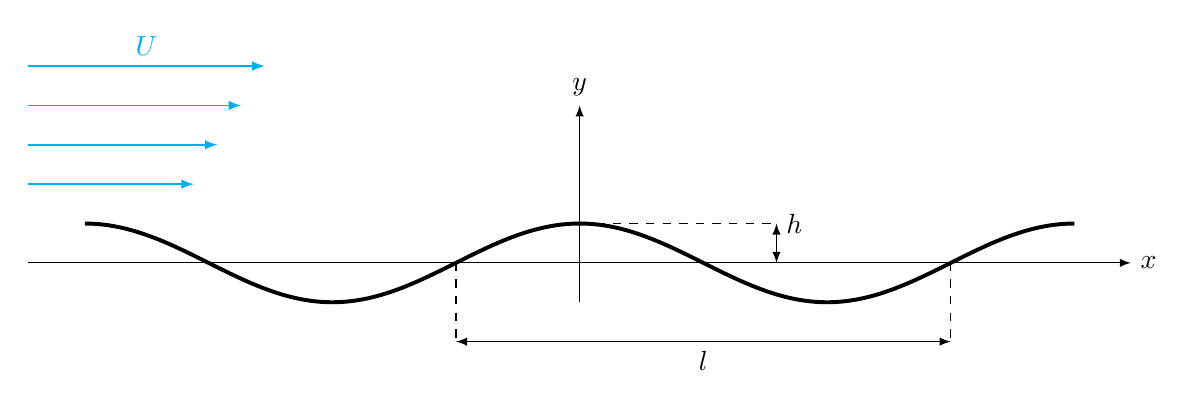
\begin{tikzpicture}[scale=1.0]
            % Achsen
        \def\startx{-7}
        \def\endx{-4}
        \def\starty{2.5}
        \def\ydis{0.5}
        \def\xenddis{0.3}
        \draw[->,>=latex] (-7, 0) -- (7, 0) node[right] {$x$};
        \draw[->,>=latex] (0, -0.5) -- (0, 2) node[above] {$y$};
        \draw[->,>=latex,cyan, line width=0.02cm] (\startx, \starty) -- (\endx, \starty) node[midway, yshift=0.25cm] {$U$};
        \draw[->,>=latex,cyan, line width=0.02cm] (\startx, \starty-\ydis) -- (\endx-\xenddis, \starty-\ydis);
        \draw[->,>=latex,cyan, line width=0.02cm] (\startx, \starty-2*\ydis) -- (\endx-2*\xenddis, \starty-2*\ydis);
        \draw[->,>=latex,cyan, line width=0.02cm] (\startx, \starty-3*\ydis) -- (\endx-3*\xenddis, \starty-3*\ydis);

        % % Gitterlinien optional
        % \draw[very thin, gray!30] (0, -1.5) grid[xstep=1, ystep=0.5] (7, 1.5);

        % Sinusfunktion
        \draw[thick, line width=0.05cm, black, domain=-2*pi:2*pi, samples=200] 
        plot (\x, {0.5*cos(\x r)});

        % Vermassungslinie l
        \def\xpos{0}
        \def\ypos{-1}
        \def\startmeas{-pi/2}
        \def\endmeas{3*pi/2}
        \draw[<->,>=latex] (\startmeas,\ypos) -- (\endmeas,\ypos) node[midway, below] {$l$};

        % Hilfslinien
        \draw[dashed] (\startmeas,\xpos) -- (\startmeas,\ypos);
        \draw[dashed] (\endmeas,\xpos) -- (\endmeas,\ypos);
        
        % Vermassungslinie h
        \def\xpos{2.5}
        \def\ypos{0}
        \def\startmeas{0}
        \def\endmeas{0.5}
        \draw[<->,>=latex] (\xpos,\startmeas) -- (\xpos,\endmeas) node[right] {$h$};

        % Hilfslinien
        \draw[dashed] (\startmeas,\endmeas) -- (\xpos,\endmeas);
        \draw[dashed] (\startmeas,\ypos) -- (\xpos,\ypos);
    \end{tikzpicture}
    }
    \caption{Strömung über einem Wellblech.
\index{Wellblech}}
    ~\label{fig:wellblech}
\end{figure}

% \end{document}

Dabei definieren wir das Potential als
\begin{align*}
    \Phi
    =
    U\,x + A\,\frac{l}{2\,\pi}\,\sin\left(\frac{2\,\pi\,x}{l}\right)
    \,e^{-\frac{2\,\pi\,y}{l}}
\end{align*}
wobei $U$ die ungestörte Geschwindigkeit im 
Unendlichen $y\rightarrow\infty$ bedeutet.

\subsection{Inkompressible Strömung}
Bei inkompressibler Strömung ist die
Laplace-Gleichung~\eqref{eq:laplace} sofort erfüllt.
Das kann bewiesen werden, indem wir für das Potential
die zweiten Ableitungen
\begin{align*}
    \frac{\partial\,^2\,\Phi}{\partial\,x^2}
    &= \frac{A\,2\,\pi}{l}\,\sin\left(\frac{2\,\pi\,x}{l}\right)
    e^{-\frac{2\,\pi\,y}{l}} \\
    \frac{\partial\,^2\,\Phi}{\partial\,y^2}
    &= -\frac{A\,2\,\pi}{l}\,\sin\left(\frac{2\,\pi\,x}{l}\right)
    \,e^{-\frac{2\,\pi\,y}{l}}
\end{align*}
berechnen wobei ersichtlich ist, dass
\begin{align*}
    \frac{\partial\,^2\,\Phi}{\partial\,x^2}
    =
    -\frac{\partial\,^2\,\Phi}{\partial\,y^2}.
\end{align*}
Es existiert dann auch eine sogenannte Stromfunktion
\begin{align*}
    \Psi
    =
    U\,y - A\,\frac{l}{2\,\pi}\,\cos\left(\frac{2\,\pi\,x}{l}\right)
    \,e^{-\frac{2\,\pi\,y}{l}},
\end{align*}
welche die Bedingung
\begin{align*}
    u 
    &=
    \frac{\partial\,\Phi}{\partial\,x}
    =
    \frac{\partial\,\Psi}{\partial\,y}
    \\
    v
    &=
    \frac{\partial\,\Phi}{\partial\,y}
    =
    -\frac{\partial\,\Psi}{\partial\,x}
\end{align*}
erfüllt.
Auch die Stromfunktion ist eine Lösung der Laplace-Gleichung
\begin{align*}
    \frac{\partial\,^2\,\Psi}{\partial\,x\,^2}
    +
    \frac{\partial\,^2\,\Psi}{\partial\,y\,^2}
    =
    0.
\end{align*}
Wenn wir $\Psi = 0$ setzen, dann erhalten wir die Gleichung
einer Stromlinie
\begin{align}
    0 = U\,y - A\,\frac{l}{2\,\pi}\,
    \cos\left(\frac{2\,\pi\,x}{l}\right)\,
    e^{-\frac{2\,\pi\,y}{l}},\label{eq:stromlinie}
\end{align}
aufgelöst nach $y$ ergibt das
\begin{align*}
    y
    =
    \frac{A}{U}\,\frac{l}{2\,pi}\,
    \cos\left(\frac{2\,\pi\,x}{l}\right)\,
    e^{-\frac{2\,\pi\,y}{l}}.
\end{align*}
Wir setzen zusätzlich 
\begin{align*}
    \frac{A}{U} \ll 1,
\end{align*}
damit näherungsweise gilt
\begin{align*}
    y
    =
    h\,\cos\left(\frac{2\,\pi\,x}{l}\right).
\end{align*}
Die Stromlinie sehr nahe am Wellblech ist eine
Kosinunslinie bzw. sie entspricht gerade der Kontur
des Blechs.
Die anderen Stromlinien $y > 0$ gehen mit zunehmendem $y$
in Gerade über, weil
\begin{align*}
    \lim_{y\,\to\,\infty}
    e^{-\frac{2\,\pi\,y}{l}}
    =
    0.
\end{align*}
Das Ganze sieht man auch in Abbildung~\ref{fig:stromlinien}.
\begin{figure}
    \centering
    \includegraphics[width=\textwidth]{papers/ueberschall/figures/Stromlinien.pdf}
    \caption{Stromlinien über dem Wellblech für $\frac{A}{U}=0.2$.}
    ~\label{fig:stromlinien}  
\end{figure}

Mit Hilfe der bernoullischen Gleichung, gemäss~\cite{BernoulliWikiDE},
\begin{align*}
    p_{\text{tot}} 
    = 
    p 
    + 
    \frac{1}{2}\,\rho\,V^2 
    + 
    \rho\,g\,z = \text{const},
\end{align*}
wobei $p_{\text{tot}}$ der Totaldruck ist, 
$\rho$ die Dichte des Fluids, $g$ die Erdbeschleunigung,
$V$ die Geschwindigkeit an einem Ort auf der Stromlinie 
und $z$ die Höhe über einem Bezugspunkt,
falls es sich um ein dreidimensionales Strömungsfeld handelt.

Da wir jedoch ausschliesslich in der $x,y$-Ebene arbeiten, 
fällt der letzte Term weg, weil $z = 0$.
Es bleibt somit:
\begin{align*}
    \underbrace{p}_{\text{statischer Druck}} 
    + 
    \underbrace{\frac{1}{2}\,\rho\,V^2}_{\text{dynamischer Druck}} 
    = 
    \text{const},
\end{align*}
was bedeutet, dass entlang einer Stromlinie 
der statische Druck und der dynamische Druck
zusammen konstant bleiben.

Wenn wir nun den lokalen Druck $p$ berechnen möchten, 
verwenden wir die freie Strömungsgeschwindigkeit $U$
als Referenzgrösse. 
Daraus ergibt sich:
\begin{align*}
    p_\infty 
    + 
    \frac{1}{2}\,\rho\,U^2 
    = 
    p 
    + 
    \frac{1}{2}\,\rho\,V^2,
\end{align*}
umgestellt nach dem lokalen Druck:
\begin{align*}
    p = p_\infty + \frac{1}{2}\,\rho\,(U^2 - V^2),
\end{align*}
wobei $V^2$ sich ergibt aus:
\begin{align*}
    V^2 = u^2 + v^2.
\end{align*}

Damit kann nun die Druckverteilung über dem Wellblech visualisiert werden, 
wie in Abbildung~\ref{fig:druckverteilung} dargestellt. 
Es handelt sich dabei um den relativen Druck, 
das heisst, der Druck ist bezogen auf den Umgebungsdruck. 
Deutlich erkennbar ist, dass der höchste Druck an den konkaven Stellen auftritt, 
während an den konvexen Stellen der niedrigste Druck herrscht.
\begin{figure}
    \centering
    \includegraphics[width=\textwidth]{papers/ueberschall/figures/Druckverteilung.pdf}
    \caption{Relative Druckverteilung über dem Wellblech.}
    ~\label{fig:druckverteilung}  
\end{figure}

\subsection{Kompressible Strömung}
Bei kompressibler Strömung gestaltet sich die Situation etwas komplexer.
Die Ausgangslage ist eine partielle Differentialgleichung zweiter Ordnung,
die durch geeignete Vereinfachungen auf jene Terme reduziert wurde, 
welche den grössten Einfluss auf die Abweichung haben.
Das genaue Vorgehen ist in~\cite{Ackeret1928} ausführlich dokumentiert.

Die folgende Gleichung stellt daher eine Näherungslösung dar,
die jedoch wesentliche Eigenschaften der exakten Lösung widerspiegelt:
\begin{align}
    \frac{\partial\,^2\,\Phi}{\partial\,x\,^2}\,
    \left(1-\frac{U^2}{a^2}\right)
    +
    \frac{\partial\,^2\,\Phi}{\partial\,y\,^2}
    =
    0\label{eq:kompressible_stroemung}
\end{align}
Der Ausdruck in der Klammer ist eine Konstante, d.h.
durch die einfache Koordinatentransformation
\begin{align*}
    x 
    &=
    \xi \\
    y\,\beta
    &=
    \eta \\
    \beta
    &=
    \sqrt{1-\frac{U^2}{a^2}}
\end{align*}
wird daraus wenig überraschend
\begin{align*}
    \frac{\partial\,^2\,\Phi}{\partial\,\xi\,^2}\,
    +
    \frac{\partial\,^2\,\Phi}{\partial\,\eta\,^2}
    =
    0
\end{align*}
die gewöhnlichen laplaceschen Gleichung, wie
bei der Potentialströmung.
Das Potential dieser kompressiblen Strömung ergibt sich zu
\begin{align*}
    \Phi
    =
    U\,x + A\,\frac{l}{2\,\pi}\,\sin\left(\frac{2\,\pi\,x}{l}\right)
    \,e^{-\frac{2\,\pi\,y\,\beta}{l}}
\end{align*}
und die dazugehörige Stromfunktion
\begin{align*}
    \Psi
    =
    U\,y - U\,\frac{h}{\beta^2}\,\cos\left(\frac{2\pi x}{l}\right)
    \,e^{-\frac{2\pi y \beta}{l}}.
\end{align*}
Durch gleiches Vorgehen wie bei Gleichung~\eqref{eq:stromlinie}
erhalten wir für $y\,\to\,0$
\begin{align*}
    y
    =
    \frac{A\,\beta\,l}{2\,\pi\,U}\,
    \cos\left(\frac{2\,\pi\,x}{l}\right).
\end{align*}
Damit wäre für kleine $y$ die Amplitude $h$ der Kosinuslinie
\begin{align*}
    h
    =
    \frac{A\,l\,\beta}{2\,\pi\,U}
\end{align*}
und somit 
\begin{align*}
    A
    =
    \frac{2\,\pi\,h\,U}{\beta\,l}.
\end{align*}
Demnach formulieren wir neu $\Phi$ als
\begin{align*}
    \Phi
    =
    U\,x + U\,\frac{h}{\beta}\,\sin\left(\frac{2\,\pi\,x}{l}\right)
    \,e^{-\frac{2\,\pi\,y\,\beta}{l}}.
\end{align*}
Der Faktor~$\beta$ beeinflusst das Abklingen der Störung,
wie in Abbildung~\ref{fig:abklingen_stromlinie} 
für drei verschiedene Fälle dargestellt ist.
Dazu werden die Stromlinien über einem Buckel visualisiert.
\begin{figure}
    \centering
    \begin{minipage}[b]{0.32\textwidth}
        \centering
        \includegraphics[width=\linewidth]{papers/ueberschall/figures/abklingen_10.pdf}
        \caption*{$\beta = 1$ ; $U = 10\,\frac{\mathrm{m}}{\mathrm{s}}$}
    \end{minipage}
    \hfill
    \begin{minipage}[b]{0.32\textwidth}
        \centering
        \includegraphics[width=\linewidth]{papers/ueberschall/figures/abklingen_200.pdf}
        \caption*{$\beta = 0.81$ ; $U = 200\,\frac{\mathrm{m}}{\mathrm{s}}$}
    \end{minipage}
    \hfill
    \begin{minipage}[b]{0.32\textwidth}
        \centering
        \includegraphics[width=\linewidth]{papers/ueberschall/figures/abklingen_340.pdf}
        \caption*{$\beta = 0$ ; $U = a$}
    \end{minipage}
    \caption{Stromlinien bei verschiedenen Strömungsgeschwindigkeiten im Unterschall.}
~\label{fig:abklingen_stromlinie}
\end{figure}

\subsection{Überschall}
Nun betrachten wir die Strömung im Überschallbereich.
Wir starten dabei bereits mit der vereinfachten 
Gleichung~\eqref{eq:kompressible_stroemung}:
\begin{align*}
    \frac{\partial^2\,\Phi}{\partial\,x^2}
    \left(1 - \frac{U^2}{a^2}\right)
    =
    -\frac{\partial^2\,\Phi}{\partial\,y^2},
\end{align*}
wobei der rechte Term zur besseren Übersicht auf die 
linke Seite verschoben wurde.

Da im Überschallbereich $U > a$ gilt, wird der Ausdruck 
in der Klammer negativ.
Es ist daher sinnvoll, die Gleichung in folgender 
Form umzuschreiben:
\begin{align*}
    \frac{\partial^2\,\Phi}{\partial\,x^2}
    \left(\frac{U^2}{a^2} - 1\right)
    =
    \frac{\partial^2\,\Phi}{\partial\,y^2}.
\end{align*}

Führen wir nun eine geeignete Koordinatentransformation durch,
\begin{align*}
    x 
    &= 
    \xi, \\
    y\,\beta 
    &= 
    \eta,
\end{align*}
mit dem Parameter
\begin{align*}
    \beta = \sqrt{\frac{U^2}{a^2} - 1},
\end{align*}
so ergibt sich die transformierte Gleichung:
\begin{align*}
    \frac{\partial^2\,\Phi}{\partial\,\xi^2}
    -
    \frac{\partial^2\,\Phi}{\partial\,\eta^2}
    =
    0.
\end{align*}
Diese Gleichung ähnelt formal der ursprünglichen Gleichung 
für den Unterschallbereich, weist jedoch ein 
unterschiedliches Vorzeichen im zweiten Term auf.
Dementsprechend handelt es sich hier um eine hyperbolische 
Differentialgleichung, die Wellenvorgänge beschreibt.
Das Strömungsverhalten im Überschallbereich ist daher — 
in gewisser Weise — mit dem Verhalten von Wellen in Wasser vergleichbar.

\input{papers/helmholtz/teilNeu01.tex}
%
% teil3.tex -- Beispiel-File für Teil 3
%
% (c) 2020 Prof Dr Andreas Müller, Hochschule Rapperswil
%
% !TEX root = ../../buch.tex
% !TEX encoding = UTF-8
%
\section{Mahtematische Grundlagen
\label{helmholtz:section:Mahtematische_Grundlagen}}
\kopfrechts{Mahtematische Grundlagen}


\subsection{Vektorfelder und Operatoren
\label{helmholtz:subsection:Vektorfelder_Operatoren}}

\subsection{Charakterisierung von Vektorfeldern
\label{helmholtz:subsection:Charakterisierung}}

\subsection{Vektoridentitäten und Integralsätze
\label{helmholtz:subsection:Vektoridentitaeten}}



%
% teil3.tex -- Beispiel-File für Teil 3
%
% (c) 2020 Prof Dr Andreas Müller, Hochschule Rapperswil
%
% !TEX root = ../../buch.tex
% !TEX encoding = UTF-8
%
\section{Die Helmholtz-Zerlegung
\label{helmholtz:section:Helmholtz_Zerlegung}}
\kopfrechts{Helmholtz-Zerlegung}


\subsection{Formale Definition der Helmholtz-Zerlegung
\label{helmholtz:subsection:def_Helmholtz_Zerlegung}}

\subsection{Mahtematischer Nachweis der Eigenschaften
\label{helmholtz:subsection:math_Nachweis}}

\subsection{Berechnung der Potentiale
\label{helmholtz:subsection:Berechnung der Potentiale}}

\subsection{Bedingungen und Eindeutigkeit
\label{helmholtz:subsection:Bedingungen_Eindeutigkeit}}



%
% teil3.tex -- Beispiel-File für Teil 3
%
% (c) 2020 Prof Dr Andreas Müller, Hochschule Rapperswil
%
% !TEX root = ../../buch.tex
% !TEX encoding = UTF-8
%
\section{Akustische Grundlagen und Feldtheorie
\label{helmholtz:section:akustische_Grundlagen}}
\kopfrechts{Akustische Grundlagen und Feldtheorie}


\subsection{Grundbegriffe der physiklalischen Akustik
\label{helmholtz:subsection:Grundbegriffe_Akustik}}

\subsection{Energiebetrachtungen in akustischen Feldern
\label{helmholtz:subsection:Energiebetrachtung}}




%
% teil3.tex -- Beispiel-File für Teil 3
%
% (c) 2020 Prof Dr Andreas Müller, Hochschule Rapperswil
%
% !TEX root = ../../buch.tex
% !TEX encoding = UTF-8
%
\section{Die komplexe Schallintensität
\label{helmholtz:section:Schallintensitaet}}
\kopfrechts{Die komplexe Schallintensität}


\subsection{Definition und Bedeutung der komplexen Schallintensität
\label{helmholtz:subsection:def_Schallintensitaet}}

\subsection{Eigenschaften der Intensitätskomponenten
\label{helmholtz:subsection:def_Schallintensitaet}}


\subsection{Mathematische Analyse der Intensitätskomponenten
\label{helmholtz:subsection:def_Schallintensitaet}}




%
% teil3.tex -- Beispiel-File für Teil 3
%
% (c) 2020 Prof Dr Andreas Müller, Hochschule Rapperswil
%
% !TEX root = ../../buch.tex
% !TEX encoding = UTF-8
%
\section{Helmholtz-Zerlegung in der Akustik
\label{helmholtz:section:Helmholtz_Zerlegung_Akustik}}
\kopfrechts{Helmholtz-Zerlegung in der Akustik}


\subsection{Zerlegung des Schallschnellefeldes
\label{helmholtz:subsection:Zerlegung_Schallschnelle}}
Angewendet auf das Schallschnellefeld $\mathbf{u}$ können wir dieses wie folgt zerlegen:
 
\begin{equation}
\underbrace{\mathbf{u}}_{\text{Schallschnellefeld}} =  \underbrace{-\nabla \Phi}_{\text{irrotationaler~Anteil}} + \underbrace{\nabla \times \mathbf{\Psi}}_{\text{solenoidaler~Anteil}}.
\end{equation}
 
\noindent Die physikalische Interpretation der Komponenten des Schallschnellefeldes lässt sich wie folgt beschreiben:
 
\begin{itemize}
\item Der irrotationale Anteil $-\nabla \Phi$ ist wirbelfrei, da die Rotation verschwindet.
\begin{itemize}
\item Dieser Anteil hat keine Rotation: $\nabla \times (-\nabla \Phi) = 0$.
\item Die Feldlinien verlaufen strahlenförmig von Quellen zu Senken.
\end{itemize}
 
\item Der solenoidale Anteil $\nabla \times \mathbf{\Psi}$ hat gemäss der Definition immer Divergenz null und wird auch quellenfrei genannt.
\begin{itemize}
\item Dieser Anteil hat keine Divergenz: $\nabla \cdot (\nabla \times \mathbf{\Psi}) = 0$.
\item Die Feldlinien bilden geschlossene Schleifen ähnlich einem Magnetfeld.
\end{itemize}
\end{itemize}

\subsection{Direkte Verbindung zur Komplexen Schallintensität
\label{helmholtz:subsection:Zerlegung_Schallschnelle}}

Wie bereits beschrieben, stellt die komplexe Schallintensität $\mathbf{I}_c$ den Energietransport in einem Schallfeld dar und lässt sich in zwei fundamentale Komponenten zerlegen:
 
\begin{itemize}
\item Aktive Intensität $\mathbf{I}$
\item Reaktive Intensität $\mathbf{Q}$
\end{itemize}
 
\noindent Die komplexe Schallintensität ist definiert als:
 
\begin{equation}
\mathbf{I}_c (\mathbf{r}) = \frac{1}{2} \: p(\mathbf{r}) \: \mathbf{u}^{*}(\mathbf{r}),
\end{equation}
 
\noindent wobei $p(\mathbf{r})$ den komplexen Schalldruck und $\mathbf{u}^{*}(\mathbf{r})$ die komplexe Konjugation der Schallschnelle $\mathbf{u}(\mathbf{r})$ beschreibt. Diese Formulierung berücksichtigt die Phasenverschiebung zwischen Schalldruck und Schallgeschwindigkeit und ermöglicht die Zerlegung des Energieflusses in quellenfreie und wirbelfreie Anteile gemäss der Helmholtz-Zerlegung.
 
Bei näherer Betrachtung ist zu erkennen, dass die komplexe Schallintensität eine ähnliche Struktur wie die Helmholtz-Zerlegung aufweist und sich wie folgt darstellen lässt:
 
\begin{equation}
\mathbf{I}_c (\mathbf{r}) = \underbrace{\mathbf{I}(\mathbf{r})}_{\frac{1}{2} \operatorname{Re} \, \{ p(\mathbf{r}) \, \mathbf{u}^*(\mathbf{r}) \}} + \underbrace{j\,\mathbf{Q}(\mathbf{r})}_{\frac{1}{2} \operatorname{Im} \, \{ p(\mathbf{r}) \, \mathbf{u}^*(\mathbf{r}) \}}.
\end{equation}
 
\noindent Es zeigt sich eine direkte Korrespondenz zwischen den Komponenten der Helmholtz-Zerlegung und der komplexen Schallintensität:
 
\begin{equation}
\mathbf{I}_c (\mathbf{r}) = \underbrace{\mathbf{I}(\mathbf{r})}_{\nabla \cdot \mathbf{I} = 0 \text{ (quellenfrei)}} + \underbrace{j\,\mathbf{Q}(\mathbf{r})}_{\nabla \times \mathbf{Q} = 0 \text{ (wirbelfrei)}}.
\end{equation}
 
\noindent Durch diese Äquivalenz können wir folgende Korrespondenz feststellen:
 
\begin{itemize}
\item Der irrotationale Anteil der Schallschnelle korrespondiert mit der aktiven Intensität.
\item Der solenoidale Anteil der Schallschnelle korrespondiert mit der reaktiven Intensität.
\end{itemize}

\subsection{Energie-Interpretation der Zerlegung
\label{helmholtz:Energie_Interpretation}}
 
Die Helmholtz-Zerlegung ermöglicht eine tiefe physikalische Interpretation der Energieverteilung und -übertragung in akustischen Feldern:
 
\begin{itemize}
\item Die aktive Intensität $\mathbf{I}(r)$ beschreibt den zeitgemittelten Netto-Energiefluss pro Fläche an dem Ort $r$ und lässt sich ausdrücken als:
\begin{equation}
\mathbf{I}(\mathbf{r}) = \frac{1}{T}\int_0^T \mathbf{I}_i(\mathbf{r},t)\,\mathrm{d}t = \frac{1}{2}\Re\left( p(\mathbf{r})~\mathbf{u}^*(\mathbf{r})\right).
\end{equation}
 
In quellenfreien, stationären Feldern ohne Energieabsorption gilt:
\begin{equation}
\nabla \cdot \mathbf{I} = 0.
\end{equation}
 
Diese Komponente ist mit dem irrotationalen Anteil des Schallschnellefeldes verknüpft und repräsentiert den tatsächlichen Energiefluss durch das Medium.
 
\item Die reaktive Intensität $\mathbf{Q}(r)$ beschreibt die zeitlich gemittelte Dichte der nicht-propagierenden, oszillierenden Energie:
\begin{equation}
\mathbf{Q}(\mathbf{r}) = \frac{1}{2}\Im\left(p(\mathbf{r})~\mathbf{u}^*(\mathbf{r})\right).
\end{equation}
 
Sie ist wirbelfrei:
\begin{equation}
\nabla \times \mathbf{Q} = 0
\end{equation}
 
Und steht in direkter Beziehung zur Differenz zwischen kinetischer Energie T und potentieller Energie V:
\begin{equation}
\nabla \cdot \mathbf{Q} = -2 \omega (T-V).
\end{equation}
 
Diese Komponente ist mit dem solenoidalen Anteil des Schallschnellefeldes verknüpft und stellt die oszillierende, lokal gespeicherte Energie dar, die nicht zum Netto-Energietransport beiträgt.
\end{itemize}
 
\noindent Anhand von zwei Extremfällen lässt sich diese Interpretation besonders gut veranschaulichen:

\begin{itemize}


 
\item Ebene Welle ($\mathbf{Q} = 0$):
Bei einer ebene Welle ist die Amplitude konstant $P(\mathbf{r}) = A = konst.$ bzw. $\nabla P = 0$, was dazu führt, dass die reaktive Intensität verschwindet. Schalldruck und Schallschnelle sind in Phase $\phi = 0^{\circ}$. Die komplexe Intensität reduziert sich zu:
 
\begin{equation}
\mathbf{I}_c (\mathbf{r}) = \mathbf{I}(\mathbf{r}) + \cancel{j\,\mathbf{Q}(\mathbf{r})}
\end{equation}
 
Die aktive Intensität ergibt sich zu: $\mathbf{I} = \frac{|\mathbf{A}|^2}{2 \rho_0 c_0}$ und zeigt in Richtung der Wellenausbreitung.
 
\item Stehende Welle ($\mathbf{I} = 0, \mathbf{Q} \neq 0$): 
Bei einer stehenden Welle überlagern sich zwei gleiche ebene Wellen mit gleicher Amplitude in entgegengesetzter Richtung. An jedem Punkt ist entweder $P = maximal$ und $\mathbf{u} = 0$. Oder $P = 0$ und $\mathbf{u} = maximal$. Schalldruck und Schallschnelle sind um 90° phasenverschoben. Die komplexe Intensität reduziert sich zu:
 
\begin{equation}
\mathbf{I}_c (\mathbf{r}) = \cancel{\mathbf{I}(\mathbf{r})} + j\,\mathbf{Q}(\mathbf{r})
\end{equation}

\end{itemize}
 
\noindent In diesem Fall gibt es keinen Netto-Energietransport, sondern nur lokale Energieoszillation.


\subsection{Visualisierung und Feldmuster
\label{helmholtz:subsection:Visualisierung}}
Die Helmholtz-Zerlegung führt zu charakteristischen Feldmustern, die sich wie folgt grafisch darstellen lassen.
 
\begin{itemize}
\item Der irrotationale Anteil bildet Quellenfelder mit radialen Feldlinien, die von Quellen ausgehen oder in Senken münden:
 
\begin{figure}
\centering
\includegraphics[width=0.8\textwidth]{papers/helmholtz/images/Quelle.png}
\caption{Quellenmuster im irrotationalen Feldanteil}
\label{fig:quelle}
\end{figure}
 
\begin{figure}
\centering
\includegraphics[width=0.8\textwidth]{papers/helmholtz/images/Senke.png}
\caption{Senkenmuster im irrotationalen Feldanteil}
\label{fig:senke}
\end{figure}
 
\item Der solenoidale Anteil bildet Wirbelfelder mit geschlossenen Feldlinien, ähnlich einem Magnetfeld.
\end{itemize}
  
\begin{figure}
\centering
\includegraphics[scale=0.6]{papers/helmholtz/images/aktiveSchallintensitaet.png}
\caption{Visualisierung des aktiven Schallintensitätsfeldes für eine Anordnung von drei Punktquellen. Die Pfeile stellen die Vektoren der aktiven Intensität dar und zeigen die Richtung des zeitgemittelten Netto-Energieflusses. In der Nähe der Quellen ist die radial wegführende Energie zu erkennen, während in den Interferenzzonen komplexe Muster, einschliesslich der Bildung von Schallintensitätswirbeln, sichtbar werden (Abbildung aus \cite{helmholtz:paper}).}
\label{fig:aktive_intensitaet_3quellen}
\end{figure}
 
\noindent Die Visualisierung der Feldmuster erlaubt eine intuitive Interpretation von Schallfeldern:
 
\begin{itemize}
\item in Bereiche mit starker aktiver Intensität zeigen Energieausbreitung und -übertragung.
\item in Bereiche mit starker reaktiver Intensität zeigen Energieoszillation ohne Nettotransport, wie sie typischerweise im Nahfeld von Schallquellen oder bei stehenden Wellen auftritt.
\item Die räumliche Verteilung von Quellen, Senken und Wirbeln erlaubt Rückschlüsse auf die zugrundeliegenden Schallquellen und Reflexionsmuster. 

\noindent Abbildung \ref{fig:aktive_intensitaet_3quellen} verdeutlicht eindrücklich, wie die Interferenz von nur drei Quellen ausreicht, um solche komplexen Wirbelmuster zu erzeugen.
\end{itemize}
 
\noindent Diese Feldmuster sind besonders wichtig für die akustische Messtechnik, da sie eine visuelle Methode zur Identifikation von Schallquellen und zur Analyse von Energieflüssen in komplexen akustischen Feldern bieten.






\printbibliography[heading=subbibliography]
\end{refsection}
